\documentclass[notitlepage, superscriptaddress]{revtex4-2}
% \documentclass[aps, prl, preprint, superscriptaddress, longbibliography]{revtex4-1}


%%%%%%%%%%%%%%%%%%%%%%%%%%%%%%%%%%%%%%%%%%%%%%%%%%%%%%%%%%%%%%%%%%%%%
\usepackage{amsmath}
\usepackage{hyperref}
\usepackage{latexsym}
\usepackage{graphicx}
\usepackage[usenames,dvipsnames]{xcolor}
\usepackage{bm}
\usepackage[normalem]{ulem}


\begin{document}

\title{SEIR-C: An epidemic model that includes contact tracing}

\author{Lynden K. Shalm}
\affiliation{Associate of the National Institute of Standards and Technology, Boulder, Colorado 80305, USA}
\affiliation{Department of Physics, University of Colorado, Boulder, Colorado, USA}


% \author{Sae Woo Nam}
% \affiliation{National Institute of Standards and Technology, 325 Broadway, Boulder, CO 80305, USA}

\begin{abstract}
The SEIR model has been widely used to study the dynamics of pandemics. Here we update the model to include the effects of contact tracing as a means to control the outbreak. We call this new model SEIR-C.
\end{abstract}
\date{\today}
\maketitle

%%%%%%%%%%%%%%%%%%%%%%%%%%%%%%%%%%%%
\section{Introduction to SEIR}
%%%%%%%%%%%%%%%%%%%%%%%%%%%%%%%%%%%%

The SEIR model relies on a set of differential equations to model the transmission dynamics of an infectious disease. A susceptible population ($S$) has some probability of coming into contact with the infected population ($I$) while they still infectious for some time ($\tau_{inf}$). Those from $S$ who have contracted the disease are then classified as having been exposed ($E$). Those who are exposed are not infectious, but rather the disease takes some time ($\tau_{inc}$) to incubate, after which point they move to the infectious population. Individuals who are in $I$ will eventually recover after a time $\tau_{inf}$. At this point they are assumed to have achieved immunity or have died. For the situation considered here, we also assume that birth rates and death rates are equal so the total population remains constant. Therefore, the total population $N$ is given by:
\begin{eqnarray}
\label{E:SEIRPop}
N = S + E + I + R.
\end{eqnarray}

In the standard SEIR model the rate of change for each of the different disease stages are given as a set of coupled differential equations:
\begin{eqnarray}
\label{E:SEIR}
\frac{dS}{dt} &=& - \beta_0 \frac{I}{N}S, \\
\frac{dE}{dt} &=& \beta_0 \frac{I}{N}S - \frac{1}{\tau_{inc}}E, \\ 
\frac{dI}{dt} &=& \frac{1}{\tau_{inc}}E - \frac{1}{\tau_{inf}}I, \\ 
\frac{dR}{dt} &=& \frac{1}{\tau_{inf}}I.
\end{eqnarray}

Here $\beta_0 = \frac{R_{0}}{\tau_{inf}}$, where $R_{0}$ is the average number of people an infectious person in $I$ will infect and is known as the reproduction number. The rate at which the exposed population increases is therefore related to how fast an infectious person spreads the disease ($\beta_{0}$) times the fraction of the population that is infectious ($I/N$) multiplied by the number of people who are susceptible ($S$).

%%%%%%%%%%%%%%%%%%%%%%%%%%%%%%%%%%%%
\section{SEIR-C}
%%%%%%%%%%%%%%%%%%%%%%%%%%%%%%%%%%%%

Here we introduce a new layer to the model that incorporates contact tracing. Contact tracing is a method of epidemic control that relies on tracing who those infected were in contact with, and then having them self-isolate. This reduces the spread of the disease as it is possible to identify and isolate those who are infectious as well as those who could potentially become infectious. Contact tracing relies on a large portion of the population participating as well as testing a substantial fraction of the population. Here we model the dynamics of contact tracing where $p_{c}$ is the fraction of the population who choose to participate, $p_t$ is the probability of an individual getting tested in a time interval $dt$, the tests take some time $\tau_{t}$ to process, and a person who tests positive and participates in contact tracing will on average notify the individuals they have been in contact with during the previous amount of time $\tau_{c}$. It is likely that those who participate in contact tracing and are notified that they may have been in contact with an infectious individual may be more likely to get tested. To account for this, those individuals may have a different probability of getting tested, $p^{c}_{t}$. A certain percentage of the tests performed will result in either a false positive ($f_{pos}$) or a false negative ($f_{neg}$). A simplified model of SEIR-C is shown in figure \ref{f:SEIR-C}. Similar to SEIR, we will assume that the total population $N$ stays constant (births = deaths), and:
\begin{eqnarray}
\label{E:SEIRPop_c}
N = S_{tot} + E_{tot} + I_{tot} + R_{tot}.
\end{eqnarray}

\begin{figure}
\centering
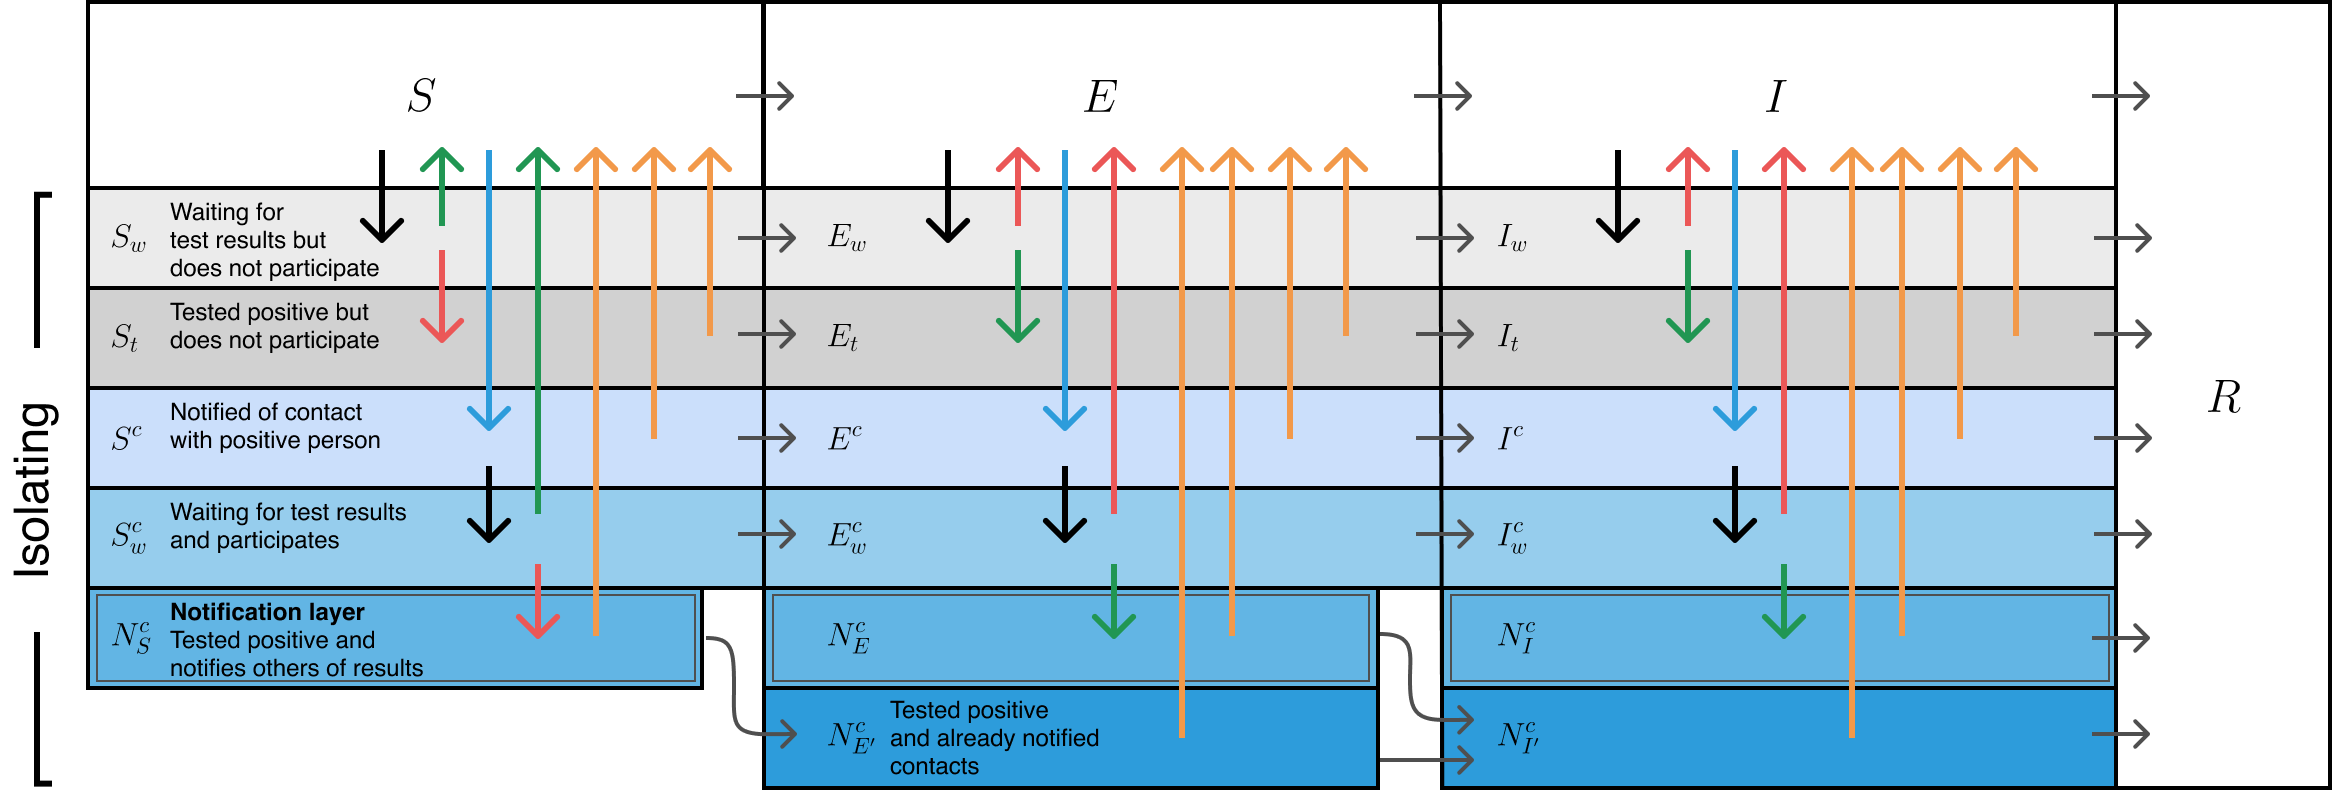
\includegraphics[width=7in]{SEIR-C_diagram.png}
\caption{\label{f:SEIR-C}
 Conceptual diagram for SEIR-C. Each of the four regions for susceptible, exposed, infectious, and recovered are separated. However, in each phase from susceptible to recovery there is a group of individuals who isolate, slowing the spread. It is convenient to divide the isolating populations in each phase into different layers. The top grey layer is for individuals who are tested and waiting for their results ($S_{w}$, $E_{w}$, or $I_{w}$), but choose not to participate in contact tracing. If they test positive, then they move to the tested population group that isolates but does not notify ($S_{t}$, $E_{t}$, or $I_{t}$). In blue represents the different layers where individuals participate in contact tracing. Those who are notified, but are not tested move into the groups $S^{c}$, $E^{c}$, or $I^{c}$. If they are tested, then while they wait for the results they move into $S^{c}_{w}$, $E^{c}_{w}$, or $I^{c}_{w}$ while waiting for the test results. If those results are positive, then they transfer to the notification layer ($N^{S}_{w}$, $N^{c}_{E}$, or $N^{c}_{I}$) where previous contacts are alerted to possible infection. Finally, those who are in a notification layer in one phase progress to either $N^{c}_{E'}$ or $N^{c}_{I'}$ to prevent them from sending a second, redundant, round of notifications to contacts. The vertical arrows represent the major population transitions within a single between the different layers. Black arrows show the movement of those who are selected for testing and are awaiting their results. Green arrows are the results of correct test results, while red arrows can represent either false positives in the susceptible phase, or false negatives in the exposure or infectious phase. Blue arrows represent contact tracing notifications (the dashed portion represents the notification, while the solid blue represents the actual population transfer). The orange layers represent population transfer from isolation layers (excluding those waiting for test results) back to the nonisolation layers after an average time of $\tau_{iso}$ has passed. The grey horizontal arrows show how subpopulations transfer between different disease phases.}
\end{figure}

To simply matters, we assume that those who are tested immediately isolate themselves while waiting for the results. If a test comes back negative then they stop isolating, and if it is positive they continue isolating. Those that are infectious ($I_{iso}$), but isolating, will have a much smaller rate of passing on the infection $\beta_{iso} = \frac{R_{iso}}{\tau_{inf}}$, while those who are infectious but have not isolating ($I$) will remain infectious at a rate of $\beta_{0}$ used in the SEIR model. Anyone who has been exposed, but is now isolating either through a contact tracing notification or because they have been tested will eventually join $I_{iso}$ after an average time of $\tau_{inc}$. 

All of those who have been exposed ($E_{tot} = E + E_{iso}$) will move to the infectious stage after an average time of $\tau_{inc}$. Similarly, all those who are infectious ($I_{tot} =  I + I_{iso}$) will eventually move to $R$ after a time $\tau_{inf}$ regardless of their testing status or whether they are isolating. For each stage we consider different sub populations. Those that are not self isolating ($S$, $E$, and $I$), those who have been notified of a possible exposure through contact tracing but have not yet been tested ($S^{c}$, $E^{c}$, and $I^{c}$), those who are waiting for test results but are not involved in contact tracing ($S_{w}$, $E_{w}$, and $I_{w}$), those who are waiting for test results and are involved in contact tracing ($S^{c}_{w}$, $E^{c}_{w}$, those who tested positive but are not involved in contact tracing ($S_{t}$, $E_{t}$, and $I_{t}$). The final group are those who are involved in contact tracing and have received a positive test result, and then notify others in $S$, $E$, and $I$ who might have been exposed. These are divided into two groups: those who receive a false positive test $N^{c}_{S}$ and those whose tests are correct $N^{c}_{E}$, $N^{c}_{I}$, and $N^{c}_{I'}$.

%%%%%%%%%%%%%%%%%%%%%%%%%%%%%%%%%%%%
\subsection{The susceptible population}
%%%%%%%%%%%%%%%%%%%%%%%%%%%%%%%%%%%%

The initial set of differential equations closely follow the SEIR model, but now account for the different infectious rates between those who are isolating and those who are not. The susceptible population, $S$, is given by:

\begin{eqnarray}
\label{E:Stot}
S_{tot} &=& S + S_{iso}, \\
% 
S_{iso} &=& S^{c} + S^{c}_{w} + S_{w} + S_{t} + N^{c}_{S},
\end{eqnarray}
where $S_{tot}$ is the total susceptible population and $S_{iso}$ is the susceptible population who are isolating. Individuals from $S_{tot}$ can move to $E$ after they come in contact with an infectious individual. The rate of infection transfer for those not in isolation ($\gamma_{0}$), and those in isolation ($\gamma_{iso}$) is given as:

\begin{eqnarray}
\label{E:infectionrates}
\gamma_{0} &=& \beta_0 \frac{I}{N} \\
% 
\gamma_{iso} &=& \beta_{iso} \frac{I_{iso}}{N}.
\end{eqnarray}

The rate of change of $S$ is determined by:
\begin{eqnarray}
\label{E:dS}
\frac{dS}{dt} &=& - [\gamma_{0}  + \gamma^{c} p_{c} +p_{t}] S + \frac{1}{\tau_{iso}}[S^{c} + S_{t} + N^{c}_{S}] + \frac{(1-f_{pos})}{\tau_{t}}[S_{w} + S^{c}_{w}].
\end{eqnarray}
The first term involve populations that leave $S$ either through infection, a notification of a possible contact with an infectious person, or selection for testing. The second term represents those who have successfully completed their isolation and return to $S$ or who test negative and return to $S$. Here the parameter $\gamma^{c}$ is a notification rate for those participating in contact tracing:
\begin{eqnarray}
\label{E:notificationrate}
\gamma^{c} &=& \frac{R^{c}}{\tau_{c}} \frac{(N^{c}_{S} + N^{c}_{E} + N^{c}_{I}) }{N}.
\end{eqnarray}
During contact tracing, the contacts in the recent past ($\tau_{c}$) that have been made by an infectious person who has tested positive are notified the need to isolate. The total population of individuals with a positive test who are participating in contact tracing is made up of those who are not infectious but received a false positive ($N^{c}_{S}$) and those who are infectious ($N^{c}_{E}$ and $N^{c}_{I}$). We assume anyone who tests positive, regardless of whether they take part in contact tracing or not, will not be retested before they recover or finish isolation. 

The population of $S_{iso}$ depends on five different populations. The rate of change of $S_{iso}$ therefore depends on the rate of change of its five constituent populations. All five of these populations have a chance of becoming infected at a rate proportional to $\gamma_{iso}$ and moving to the exposed stage. First we consider those who go into isolation because they are tested but do not participate in contact tracing. The group waits for their test results. If the results are negative, they return to $S$ but if they receive a false positive they are moved to $S_{t}$:
\begin{eqnarray}
\label{E:dS_iso}
\frac{dS_{w}}{dt} &=& p_{t} (1 -p_{c}) S - [\frac{1}{\tau_{t}}  + \gamma_{iso}] S_{w}, \\
%
\frac{dS_{t}}{dt} &=& \frac{f_{pos}}{\tau_{t}} S_{w} - [\frac{1}{\tau_{iso}}  + \gamma_{iso}] S_{t}
\end{eqnarray}
While in $S_{w}$ or $S_{t}$ there is a chance of becoming infected and moving to the exposed stage. Since everyone that is susceptible is by definition not a carrier of the illness, any positive tests must be due to false positives. The remaining susceptible populations are $S^{c}$, $S^{c}_{w}$, and $N^{c}_{S}$:
\begin{eqnarray}
\label{E:dSc}
 \frac{dS^{c}}{dt} &=& \gamma^{c} p_{c} S -[p_{t} +\frac{1}{\tau_{iso}} +\gamma_{iso}] S^{c}, \\
 %
 \frac{dS^{c}_{w}}{dt} &=& p_{t}p_{c} S + p^{c}_{t} S^{c} - [\frac{1}{\tau_{t}}  + \frac{1}{\tau_{iso}}  + \gamma_{iso}] S^{c}_{w}, \\ 
 %
 \frac{dN^{c}_{S}}{dt} &=& \frac{f_{pos}}{\tau_{t}} S^{c}_{w} - [\frac{1}{\tau_{iso}}  + \gamma_{iso}] N^{c}_{S}.  
\end{eqnarray}
Individuals who are notified through contact tracing to isolate are moved to $S^{c}$. Leaving $S^{c}$ occurs when an individual is selected for testing (moved to $S^{c}_{w}$), they become infected (move to $E^{c}$), or they finish isolation and return to $S$. The final susceptible population, $N^{c}_{S}$, are those who participate in contact tracing and receive a false positive test. This group will self isolate, and may become infectious (moving them to $E^{c}$ as they have not notified anyone since they became truly infected, but are still isolating due to the earlier false positive test). Once their isolation is finished they return to $S$.

%%%%%%%%%%%%%%%%%%%%%%%%%%%%%%%%%%%%
\subsection{The exposed population}
%%%%%%%%%%%%%%%%%%%%%%%%%%%%%%%%%%%%
The next phase in the model are those who have been exposed ($E_{tot}$). The total exposed population grows based on the number of infections caused in those susceptible, but is reduced by those who become infectious after the incubation period, $\tau_{inc}$, is over. The total population $E_{tot}$ is given by:
\begin{eqnarray}
\label{E:Etot}
E_{tot} &=& E + E_{iso}, \\ 
%
E_{iso} &=& E^{c} + E^{c}_{w} + E_{w} + E_{t} + N^{c}_{E}
\end{eqnarray}

The rate of change of $E$, the exposed population not isolating, is determined by:
\begin{eqnarray}
\label{E:dE}
\frac{dE}{dt} &=& \gamma_{0}S  + \frac{1}{\tau_{iso}}[E^{c} + E_{t} + N^{c}_{E} + ^N{c}_{E'}] + \frac{f_{neg}}{\tau_{t}}[E_{w} + E^{c}_{w}] -  [\gamma^{c} p_{c} +p_{t} + \frac{1}{\tau_{inc}}] E.
\end{eqnarray}
$E$ grows in size due to infections from S, as well as individuals who individuals who are exposed but finish their isolation ($E^{c} + E_{t} + N^{c}_{E}$), and those that are exposed but register a falser negative when tested. $E$ is diminished by those who are notified through contact tracing that they need to isolate, those that are selected for testing, and those that become infectious and move to the next phase. Most of the following equations for the exposed population also feature a rate $\frac{1}{\tau_{inc}}$ that moves them to the infectious phase.

Similar to the $S_{iso}$, $E_{iso}$ is composed of five different subpopulations. First we consider those who are not participating in contact tracing, but are selected for testing. This group moves from $E$ to $E_{w}$ where they await their test results for an average time of $\tau_{t}$. If the test results come back positive, they move to $E_{t}$ and no one is notified. If there is a false negative, they return to $E$:
\begin{eqnarray}
\label{E:dE_w}
\frac{dE_{w}}{dt} &=& \gamma_{iso} S_{w} + p_{t} (1 - p_{c}) E - [\frac{1}{\tau_{t}}  + \frac{1}{\tau_{inc}}] E_{w}, \\
%
\frac{dE_{t}}{dt} &=& \gamma_{iso} S_{t} + \frac{(1- f_{neg})}{\tau_{t}} E_{w} - [\frac{1}{\tau_{iso}}  + \frac{1}{\tau_{inc}}] E_{t}.
\end{eqnarray}
Both of the populations $E_{w}$ and $E_{t}$ also grow from people in their counterpart susceptible populations becoming infected and moving to the exposed stage (the $\gamma_{iso}$ terms). 

There are three groups who are exposed and are also participating in contact tracing. Their dynamics are governed by:
\begin{eqnarray}
\label{E:dEc}
 \frac{dE^{c}}{dt} &=& \gamma_{iso} S^{c} + \gamma^{c} p_{c} E -[p_{t} +\frac{1}{\tau_{iso}} + \frac{1}{\tau_{inc}}] E^{c}, \\
 %
 \frac{dE^{c}_{w}}{dt} &=& \gamma_{iso} S^{c}_{w} + p_{t}p_{c} E + p^{c}_{t}E^{c} - [\frac{1}{\tau_{t}}  + \frac{1}{\tau_{iso}}  + \frac{1}{\tau_{inc}}] E^{c}_{w}, \\ 
 %
 \frac{dN^{c}_{E}}{dt} &=&  \frac{(1-f_{neg})}{\tau_{t}} E^{c}_{w} - [\frac{1}{\tau_{iso}}  + \frac{1}{\tau_{inc}}] N^{c}_{E}, \\ 
 %
\frac{dN^{c}_{E'}}{dt} &=&  \gamma_{iso} N^{c}_{S} - [ \frac{1}{\tau_{iso}} + \frac{1}{\tau_{inc}}] N^{c}_{E'}. 
\end{eqnarray}
Here $E^{c}$ are the individuals who are exposed and have been notified through contact tracing to isolate, but have not yet been tested. The second group is composed of those participating in contact tracing who are awaiting test results for a time $\tau_{t}$. If the test result is a false negative they return to $E$. Otherwise, they are moved to $N^{c}_{E}$ and their contacts are notified. Finally, there are those who were in $N^{c}_{S}$ due to a false positive, but subsequently become infected. They move to $N^{c}_{E'}$ where no notifications take place (as that already occurred) and they continue to isolate. Individuals in $N^{c}_{E}$ and $N^{c}_{E'}$ can return to $E$ if their isolation period ends or if they become infectious.

%%%%%%%%%%%%%%%%%%%%%%%%%%%%%%%%%%%%
\subsection{The infectious population}
%%%%%%%%%%%%%%%%%%%%%%%%%%%%%%%%%%%%

After the incubation period, a person moves to the infectious phase where they can now infect individuals in the susceptible population. Here $I_{tot}$ is given by:
\begin{eqnarray}
\label{E:Itot}
I_{tot} &=& I + I_{iso}, \\ 
%
I_{iso} &=& I^{c} + I^{c}_{w} + I_{w} + I_{t} + N^{c}_{I} + N^{c}_{I'}.
\end{eqnarray}
 Those who are infectious, but are not isolating fall in ($I$), whose rate of change is governed by:
\begin{eqnarray}
\label{E:dI}
\frac{dI}{dt} &=& \frac{1}{\tau_{inc}}E  + \frac{1}{\tau_{iso}}[I^{c} + I_{t} + N^{c}_{I} + N^{c}_{I'}] + \frac{f_{neg}}{\tau_{t}}[I_{w} + I^{c}_{w}] -  [\gamma^{c} p_{c} +p_{t} + \frac{1}{\tau_{inf}}] I.
\end{eqnarray}
In this equation, and all the subsequent infections equations, the population grows in part from those who are exposed becoming infected after a time $\tau_{inc}$. The population also grows from those who are infectious but falsely test negative and those who are infectious but who finish isolating too early. The population of $E$ decreases either through testing, contact tracing notification, or individuals who recover at a rate of $\frac{1}{\tau_{inf}}$. 

The portion of $I_{tot}$ that is isolating is made up of six different subpopulations whose dynamics are similar to their counterparts in the exposed phase. First we have those who do not participate in contact tracing, but are isolating through testing. This group first moves from $I$ to $I_{w}$ while they wait for their test results. Individuals in the exposed group $E_{w}$ who are waiting for their test results but become infectious end up joining this population. After an average time $\tau_{t}$ the tests are complete and the individuals who test positive move to $I_{t}$ where they continue isolating or they return to $I$ if there is a false negative. Members from these two groups can also recover ($R$) after an average time $\tau_{inf}$:
\begin{eqnarray}
\label{E:dI_w}
\frac{dI_{w}}{dt} &=& \frac{1}{\tau_{inc}} E_{w} + p_{t} (1 - p_{c}) I - [\frac{1}{\tau_{t}}  + \frac{1}{\tau_{inf}}] I_{w}, \\
%
\frac{dI_{t}}{dt} &=& \frac{1}{\tau_{inc}} E_{t} + \frac{(1- f_{neg})}{\tau_{t}} I_{w} - [\frac{1}{\tau_{iso}}  + \frac{1}{\tau_{inf}}] I_{t}. 
\end{eqnarray}


%%%%%%

Finally, we have the rate equations for those who are infectious and participating in contact tracing:
\begin{eqnarray}
\label{E:dIc}
 \frac{dI^{c}}{dt} &=& \frac{1}{\tau_{inc}} E^{c} + \gamma^{c} p_{c} I -[p_{t} +\frac{1}{\tau_{iso}} + \frac{1}{\tau_{inf}}] I^{c}, \\
 %
 \frac{dI^{c}_{w}}{dt} &=& \frac{1}{\tau_{inc}} E^{c}_{w} + p_{t}p_{c} I + p^{c}_{t}I^{c} - [\frac{1}{\tau_{t}}  + \frac{1}{\tau_{iso}}  + \frac{1}{\tau_{inf}}] I^{c}_{w}, \\ 
 %
 \frac{dN^{c}_{I}}{dt} &=&  \frac{(1-f_{neg})}{\tau_{t}} I^{c}_{w} - [\frac{1}{\tau_{iso}}  + \frac{1}{\tau_{inf}}] N^{c}_{I}, \\
 %.
 \frac{dN^{c}_{I'}}{dt} &=&  \frac{1}{\tau_{inc}} [N^{c}_{E} + N^{c}_{E'}] - \frac{1}{\tau_{inf}}N^{c}_{I'}.
\end{eqnarray}
Those who are notified through contact tracing, but have not yet been tested join $I^{c}$. Those who are participating in contact tracing and are selected for testing move to $I^{c}_{w}$ where they wait for their test results an average time of $\tau_{t}$. A positive test result moves them to the notification layer $N^{c}_{I}$ where their contacts are notified. Finally, those who tested positive in $N^{c}_{E}$ (where they performed the relevant notifications) move instead to $N^{c}_{I'}$ to ensure they don't trigger a second round of notifications when they become infectious.

%%%%%%%%%%%%%%%%%%%%%%%%%%%%%%%%%%%%
\subsection{The recovered population}
%%%%%%%%%%%%%%%%%%%%%%%%%%%%%%%%%%%%

The total recovered rate are identical to that from the standard SEIR model,
\begin{eqnarray}
\label{E:dRtot}
% \frac{dI_{tot}}{dt} &=& \frac{1}{\tau_{inc}}E_{tot} - \frac{1}{\tau_{inf}}I_{tot}, \\
%
\frac{dR_{tot}}{dt} &=& \frac{1}{\tau_{inf}}I_{tot}.
\end{eqnarray}
As a reminder, it is assumed that those who recover are either immune or dead, and therefore cannot rejoin the susceptible population. 

% \bibliography{}


\end{document}


